\documentclass{acm_proc_article-sp}

\begin{document}
%
% --- Author Metadata here ---
%\conferenceinfo{WOODSTOCK}{'97 El Paso, Texas USA}

\setpagenumber{50}

%\CopyrightYear{2002} % Allows default copyright year (2002) to be over-ridden - IF NEED BE.
%\crdata{0-12345-67-8/90/01}  % Allows default copyright data (X-XXXXX-XX-X/XX/XX) to be over-ridden.
% --- End of Author Metadata ---

\title{Konfidi\titlenote{\textit{Konfidi} is the Esperanto term for trust.  
A universal concept in a universal language seemed appropriate for what we hope will become a universal system.}\titlenote{The name Konfidi applies to our system as a whole.  The various components, FOAFServer, TrustServer, and Clients, will be called by their individual names.}: Trust Networks Using PGP and RDF}
% the first note is cheesy, I admit.  can you think of a better way to say it?
% There's probably a better way to say this stuff (second stuff).  do you get the idea?
% why don't we just say the 2nd stuff at the beginning of the Konfidi section?  or not at all.  do you suspect confusion?

\numberofauthors{2}

\author{
\alignauthor Dave Brondsema\\
       \affaddr{Calvin College}\\
       \affaddr{3201 Burton SE}\\
       \affaddr{Grand Rapids, MI 49546}\\
       \email{dave@brondsema.net}
\alignauthor Andrew Schamp\\
       \affaddr{Calvin College}\\
       \affaddr{3201 Burton SE}\\
       \affaddr{Grand Rapids, MI  49546}\\
       \email{schamp@gmail.com}
}

\date{4 May 2005}

\maketitle
\begin{abstract}
We ought to write this last.
\end{abstract}

\terms{source, sink, concatenation, aggregation}

\keywords{Semantic Web, trust network, FOAF, RDF, PGP, GPG, reputation, propogation, distributed, inference, delegation, social network}

\section{Introduction}
As more and more information becomes available on the internet, there is a growing problem determining which information is reliable and accurate.  A person may, over time, develop a reputation as a reliable source of information for a certain topic, however, someone unfamiliar with that person's reputation may either place too much or too little trust in that person.  

Ratings system for reputation within certain domains (eBay auctions, for example), may be of some limited use, however, they may also be susceptible to floods of manipulative ratings.  Even if such systems can be guarded against such attacks, why should someone base whether they trust anotehr person on opinions given by others that they neither know nor trust?

A solution growing in popularity is that of creating a network of trust between individuals who know one another and have good reason to trust the ratings they give of others.  However, these systems too can subject to problems if someone impersonating a trusted party provides incorrect data boosting the reputation of an untrustworthy party.  The PGP web of trust provides the necessary verification of an individual's identity; however, it does not allow the expression of any additional information about that individual's trustworthiness on matters apart from personal identification.

In this paper, we will describe some difficulties in integrating these two kinds of trust networks, and how we designed a system to overcome them.  We will then describe our structure for representing trust data, and our methods for making trust inferences on this data.  Finally, we will discuss the software we have begun to develop so that this trust network can be put to use.

\section{Related Work}

\subsection{Representing Trust Relationships}
There seems to be a general lack of psychological research on representing trust relationships and making inferences for unspecified relationships. In fact, most work in the fields of mathematics and computer science seem to adopt an arbitrary model appropriate to the algorithm under consideration. As Guha points out\cite{guha04propagation}, there are compelling reasons for a trust representation scheme to express explicit distrust as well as trust.

For Konfidi, we have likewise has chosen an arbitrary model, but in designing the system we have made every effort to allow for adaptation to different models as research in this area develops. 

\subsection{Trust Networks and Inferences}
There are a number of papers about different propagation strategies for weighted, directed graphs\footnote{See such-and-such, and so-and-so, for example}.  For the most part, however, they are concerned with describing the networks mathematically, and do not have much in the way of practical application. 

Belief in statements vs. trust in people.

Jennifer Golbeck, at the University of Maryland, is doing graduate research on trust and reputation systems\cite{golbeckSite} that is similar to our work on this project.  Like us, she uses an extension of FOAF to represent trust relationships and a rating system\footnote{Though both our ontologies and are ratings are different in significant ways, which we will address later.}.  She has written a number of papers\footnote{list of Golbeck papers here}, and created TrustMail\cite{trustMail}, a modified email client that uses the trust network that she is building.  She is more concerned with an academic approach than a pragmatic one, since this field is still growing rapidly and she prefers to help determine a good system of standards in the area.

\subsection{The Semantic Web}
In addition to Golbeck's work, a number of others have explored the usefulness and implications of expressing trust relationships in the Semantic Web.

\subsubsection{Friend of a Friend (FOAF)}
\label{foaf}
The FOAF project\cite{foafProject} is an RDF vocabulary used to represent personal data and interpersonal relationships for the Semantic Web.  Users created RDF files describing Person objects which can specify name, email address, and so on, but more importantly, they can express relationships between Person objects.  

\subsubsection{FOAF Whitelisting}
Dan Brickley has made a non-academic attempt to investigate the use of FOAF, particularly the mbox\_sha1 property, to automatically generate email whitelists. By hashing the sender's address using SHA1, privacy is protected (and the address cannot be gathered by spiders), and so users can share whitelists of non-spam emailers. Then for all incoming mail, the sending address is hashed and the whitelist searched for the resulting value, and then is filtered accordingly. This use of FOAF is promising, but since it is localized, it is difficult for updates to propagate\cite{foafWhitelisting}. No effort was taken in this project to verify the sender's identity.

\subsection{Email Filtering by Inferred Trust}
Boykin and Roychowdhury discuss ways to infer a relationship based on existing data (From:, To:, Cc: headers)\cite{boykin04email}. This seems to work fairly well but there is often not enough data to make the spam/not-spam decision because it is based only on the user's own previously recieved messages. They clearly state a cryptographic solution would be ideal to verify identity.

\subsubsection{Spam Filtering}
Domain-level solutions, such as SPF and DomainKeys, are mostly to prevent phishing and also assume that a domain's administrator can control and monitor all its user's activities. Greylisting and blacklisting often have too many false positives and false negatives. User-level filtering, which Konfidi does in the context of email filtering, is not very common. Challenge-response mechanisms to build a whitelist are tedious for the sender and reciever and do not validate authenticity. Content-level testing is the most common, but bayesian filtering and other header checks are reactionary and must be continuously updated, and are becoming less effective as spammers create emails that look more and more real. 

\subsection{Trust Inference Using PGP}
\label{earlierPGP}
One possible approach is to use the PGP web-of-trust to filter email spam at the client's end. For example, a mail client plugin could filter incoming mail, and check to see if there was a path from the sender to the recipient, in which the recipient had signed someone's key, who had signed another key, which eventually lead to the sender's key. If there was a path within a certain length, the message would be marked as trusted, if not, it would be marked as not trusted. This approach required that most users digitally sign email messages, and it depended on users to be aware of known spammers and keep from signing their keys. However, the recommended PGP keysigning practices require only the careful verification of the key-holder's identity, and a signed key does not entail anything about trustworthiness in other areas.  Whether a user should be trusted to send good email, and not spam, is information over and above that expressed in the PGP web-of-trust itself, so the web-of-trust would be inadequate to encode such information.

A more serious flaw in an approach that depends so heavily on the client software is this:  because information about key signatures is stored as a part of the key that was signed, and not that of the signer, paths between users can only be constructed from the sender backward to the recipient. When a key is retrieved from a keyserver, all of the signatures on that key are included with it, showing which keys have signed that key, and providing a number of possible links in a chain. However, using the existing keyserver infrastructure, there is no easy way to tell which other keys a particular key has signed. If these paths are built backward using a breadth-first search from the sender to the recipient, a spammer or other malicious user could generate a large number of fake keys that are inter-signed, and then use these keys to sign the sender's key. By adding this artificial information, the client's searching capabilities would be crippled, and the web-of-trust would be polluted with fabricated keys, users, and signatures. The PGP system of key-signing and verification was designed to be robust against this sort of impersonation, by requiring photo-identification and fingerprint exchange before any key-signing, but a deluge of false information would put undue strain on the keyserver infrastructure, and would amount to a denial-of-service, of sorts.

\subsubsection{Wotsap}
\label{wotsap}
Talk about wotsap a bit.

\section{Motivation}
% moved this section heading down one paragraph.  seemed to fit better.  But we need a better opening to this paragraph then.
So, for our idea to be viable, it must first deal with these two issues, namely, representing trust information not directly in the PGP web-of-trust but rather in some other system closely coupled with it, and not being susceptible to denial-of-service attacks caused by generated false webs. We had other requirements, too. A system like this must be widely (even universally) adopted in order to be useful. As such, it must be easy for the technically unsavvy, like Aunt Sally, to use, while at the same time avoiding any diminished security stemming from being easy-to-use. It must also be available in any of the many widely-used email clients. 

\section{Konfidi}
\begin{figure*}
\centering
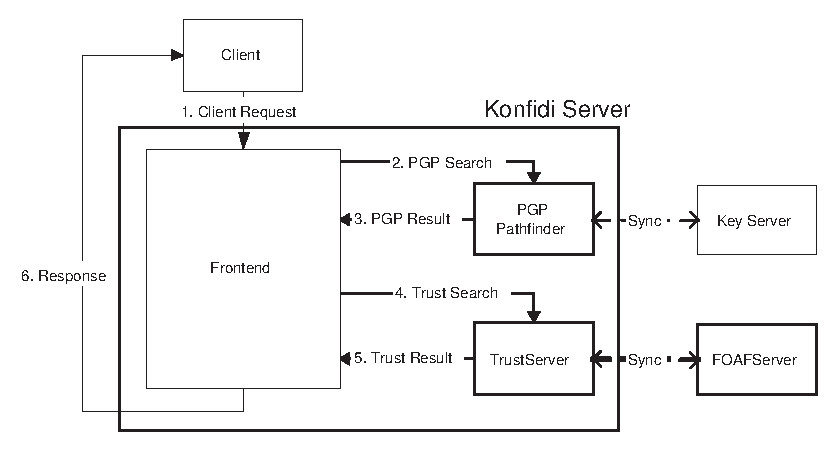
\epsfig{file=arch.eps}
\caption{The Konfidi Architecture}
\end{figure*}

\begin{figure*}
\centering
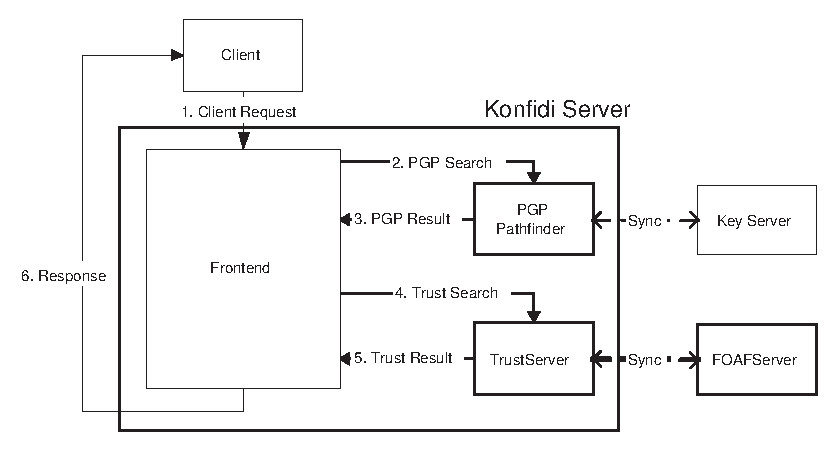
\psfig{file=arch.ps}
\caption{The Konfidi Architecture}
\end{figure*}

\subsection{Trust Ontology}
% representation is seperate from algorithm result, right?  Need to fix this paragraph if so
% what do you mean?  I suppose the algorithm can perform whatever operation on the values it wants, but I think the point is that the domain and range of the network is the same:  an inferred trust rating should look no different from an explicit one.  maybe this is unclear...
In the current research on trust inference networks, there seem to be two general kinds of representations:  one that used discrete values for varying levels of trust and returned a discrete binary (yes or no) answer, or one which used a (theoretically) continuous range of trust values and returned an answer within that range.  Now, either kind of representation could be roughly mapped onto the other, however, a continuous range would allow more finely-grained control over the data.  Further, the inferred trust values returned by searches would be similar to the explicit trust values users provided when specifying trust relationships.  This makes it easier to evaluate such results on a scale that has some familiarity.

\subsubsection{Distrust}
% shouldn't start out with "This" (I assumed it referred to the section title, Distrust).  I don't even know what concept it really is supposed to refer to
This is closely related to another important concern, that the representation give some account of distrust.  If the trust network contained values ranging from neutral trust to complete trust, then everyone in the network is trusted, explicitly, or by inference on some level at or above neutral.  If the system makes a trust inference between Alice and Bob at one level, but Alice really trusts Bob at a different level, she can explicitly state this previously implicit trust to have a more accurate result (for herself and for others who build inference paths of whom she is a member).  But, suppose that Alice feels strong negative feelings about Bob.  In this case, she would still only be able to represent this relationship as one of neutral trust.  So, the trust network must account for distrust in some reasonable way.
% refer to samples from diagram

One of the difficulties of using explicit distrust in an inference network, however, is that it is unclear how inferences should proceed once a link of distrust has been encountered.  Suppose Alice distrusts Bob, and Bob distrusts Clara.  As Guha points out\cite{guha04propagation}, there are at least two interpretations of this situation.  On the one hand, Alice might think something like "the enemy of my enemy is my friend" and so decide to put trust in Clara.  On the other hand, she might realize that if someone as scheming as Bob distrusts Clara, then Clara must really be an unreliable character, and so decide to distrust Clara.  Further, suppose Bob expressed trust for Dave.  At first consideration, it might seem reasonable to simply distrust everyone that Bob distrusts, including Dave.  But suppose there were another path through different nodes indicating some minimal level of trust for Dave.  Which path should be chosen as one which provides the correct inference?

One solution to this problem is simply to not traverse beyond a relationship of distrust, and to seek an alternate path.  There is no clear answer regarding the statements a distrusted person makes, so it is best not to consider them at all.
% multiple paths is different than distrust.  Move the following elsewhere
To overcome the problem of chosing the correct path for the inference, some kind of weighted average can be taken of all of the paths between Alice and Dave, thereby producing an answer according to whether the majority of people in the neighborhood Dave trust him or not.

We explored a method similar to this one, but in the absence of sufficient psychological research affirming a model of this type, we sought a simpler solution.  In the end, we decided on a model that corresponds to another intuition about how trust works between people, that it is more of a continuum of both trust and distrust than a measure of just one or the other.  For example, if Alice trusts Bob at some moderate level (say, .75 of a scale of 0 to 1), then it seems that she also \textit{distrusts} him at some minimal level (say, .25).  If Alice trusts Bob neutrally, then she trusts him about as much as she distrusts him.  If she distrusts him completely, then she doesn't trust him at all.  But in all of these cases, there is a trade-off between trust and distrust.  Only in the extremes is either of them eliminated completely.  So, we decided that our trust model should represent a range of values from 0 to 1, treating 0 as complete distrust, 1 as complete trust, and 0.5 as neutral, and calculate trust inferences accordingly\footnote{This also makes many propagation algorithms simpler, as we'll discuss later.}.

\subsubsection{Trust Topics}
If other attributes about a trust relationship could be expressed, in addition to the rating system, then a system like Konfidi would be useful in many wider scopes than email spam prevention.  The most important of these is the trust topic, or in other words, what the trust is about.  A natural feature of interpersonal trust relationships is that there can be many different aspects of the same trust relationship.  

(you can make an Alice-Bob-Clara-Dave diagram for this business)

For example, suppose Bob is a master chef, but is terribly gullible about the weather forecast.  Alice, of course, knows this, and so wants to express that she trusts Bob very highly when he gives advice for making souffle, but she does not trust him at all when he volunteers information about the likelihood of the next tornado.  Suppose she only knows Bob in these two capacities.  Any trust inference system should not average the two trust values and get a somewhat neutral rating for Bob, for that would lose important information about each of those two trust ratings\footnote{In fact, it would lose the only information that made these ratings useful in the first place.}.

Suppose also that, given only the above trust ratings, the system tried to make an inference on a subject that was not specified.  Perhaps Alice has some general level of trust for Bob that should be used when there is no specific rating for the topic in question.  See the discussion in Future Work for our proposal for a hierarchical system of topics that might account for this situation.

\subsubsection{Rating System}
\label{rating}
% "Rating System" seems inappropriate.  How about "Data structure" or something?
With these considerations in mind, we found that a relationship-based model would meet our needs while avoiding some of the disadvantages of other representations.  According to this system, each trust relationship is an object, and the trusting person and the trusted entity (typically a person) are specified as such\footnote{Thus, each relationship is one-way, but since the truster is responsible for the accuracy of the information, that is fine.}.  Trust relationships also have trust items specified.  Each items is composed of a topic and a numerical rating.  Each rating is on a scale from 0 to 1 inclusive, with 0 representing complete distrust, 1 representing complete trust, and 0.5 representing neutral.

Because the trust relationship is represented as its own object, other attributes may be added later, such as the dates the relationship began, annotations, etc. as the need arises.

\subsubsection{OWL Schema}
% we need to say more at some point about FOAF, so that it is clear how we are using it and why.  But where?  In related work?  Here?  I'll put it here for now.
As the FOAF project grows in popularity, an infrastructure is growing to support it, as mentioned in \ref{foaf}.  Since there would be many advantages to tapping into this infrastructure, and since the specification of trust relationships fits in naturally alongside the existing \texttt{foaf:knows} property, Konfidi also uses the Resource Description Framework (RDF)\cite{rdf} for representing trust relationships.  In addition to the FOAF vocabulary, there is a vocabulary called WOT defining and describing singing and assurance, which provides the necessary structure for associating persons and organizations with key fingerprints\cite{wot}.  By designing Konfidi's vocabulary to make use of FOAF and WOT vocabulary elements, then, we can take advantage of the established standards and make our extensions compatible with existing FOAF-enabled tools.

Konfidi uses the Web Ontology Language (OWL)\cite{owl} to define the RDF elements that make up the Konfidi trust ontology.  OWL builds on the existing RDF specification by providing a vocabulary to describe properties and classes, and their relations.  The Konfidi trust ontology provides two objects and five properties, which, in conjunction with the existing FOAF and WOT vocabularies, are sufficient to describe the trust relationships that Konfidi requires.

% how should we describe the ontology?  how about this for now?

The primary element is \texttt{Relationship}\footnote{According to RDF standards, the names of objects are capitalized, while the names of properties remain lowercase.}, which represents a relationship of trust that holds between two people.  There are two properties required for every \texttt{Relationship}, \texttt{truster} and \texttt{trusted}, which indicate the two parties to the relationship.  Both \texttt{truster} and \texttt{trusted} have \texttt{foaf:Person} objects as their targets\footnote{These \texttt{Person} objects should also contain at least one \texttt{wot:fingerprint} property specifying the PGP fingerprint of a public key held by the individual the \texttt{Person} describes.  This property is required for verification; if no \texttt{fingerprint} is available, then Konfidi cannot use the relationship.}, which may be defined in the same file, inline, or in external documents indicated by their resource URIs\footnote{Because it does not matter where the \texttt{foaf:Person} data is stored, users may keep files indicating trust relationships separate from main FOAF files.  However, to prevent spoofing, any file containing one or more \texttt{Relationship} objects must have a valid signature from a public key \texttt{fingerprint} corresponding to each \texttt{Person} listed as a \texttt{truster} in that file.  As described in \ref{foafserver}, flexibility in data location can have a number of advantages. }.  

In addition to \texttt{truster} and \texttt{trusted}, each \texttt{Relationship} requires at least one \texttt{about} property, which relates the trust \texttt{Relationship} to a trust \texttt{Item}\footnote{A \texttt{Relationship} is not limited in the other properties it can have, so auxiliary information about the relationship, such as when it began, who introduced it, etc. may be recorded without having an effect on the requirements of Konfidi.}.  Each \texttt{Item} has two properties belonging to it.  The \texttt{topic} property specifies the subject of the trust according to a trust topic hierarchy\footnote{yet to be developed} and the \texttt{rating} property indicates the value, according to the 0-1 scale specified in Section~\ref{rating} of the trust assigned to the relationship on that topic.  

A \texttt{Relationship} may have more than one \texttt{Item} that it is about.  For example, remember the example given above, in which Alice trusts Bob highly about cooking, and distrusts him somewhat about the weather.  This might be represented in our ontology as something like the following\footnote{That is, supposing that the objects \texttt{alice123}, \texttt{bob1812}, \texttt{cooking}, and \texttt{weather} are all defined elsewhere in the same file.}.  For a more in-depth example, see Appendix~\ref{trustExample}.:

\begin{verbatim}
<Relationship>
  <truster rdf:resource="#alice123" />
  <trusted rdf:resource="#bob1812" />
  <about>
    <Item>
      <rating>.95</rating>
      <topic rdf:resource="#cooking" />
    </Item>
  </about>
  <about>
    <Item>
      <rating>.35</rating>
      <topic rdf:resource="#weather" />
    </Item>
  </about>
</Relationship>
\end{verbatim}

See Appendix~\ref{schemaCode} for the full OWL source code.

\subsection{FOAFServer}
\label{foafserver}
% in the "owl schema" section, I say that this section talks about the advantages of having distributed FOAF and RDF records, so be sure to cover that here as part of hte motivation of the Foafserver.  you remember what I mean, right?

% explain that this is not part of Konfidi proper, but a requisite system like PGP keyservers are

As Konfidi developed, it seemed that two important but separate components were needed to fulfill the two major needs of our project.  First, we needed a way to store data specifying trust relationships.  Second, we needed a way to represent the network specified in the data, and traverse it to calculate trust values.

One need was for a system to store trust network data, verify signatures on that data, and allow for updates of existing files and their signatures.

If Konfidi were to be useful as a system of trust management, then the operations it performs and the results it returns must be trusted by the users.  Thus, to prevent malicious users from submitting faulty or incorrect trust data for others, Konfidi will require every file submitted to be digitally signed by the key of the user who is indicated as the trusting party.  Konfidi will then verify the signature before accepting the data as legitimate and passing it along to the trust management system.

URI based lookup

communications with trust server and the requirements for a completely trusted system (e.g., signed communication at every step, or something)

\subsection{TrustServer}
This part of the design is the core element of Konfidi.  Storing and managing the data would not be of much use in this context unless we did something with it.  So, the TrustServer would handle requests for trust ratings, verify that a PGP connection exists, and traverse the internal representation to find a path.  Since these three tasks are so distinct, all of Konfidi is divided into three parts, a frontend which listens for requests and dispatches them, and two backend components, one to search the PGP web-of-trust and another to query against Konfidi's own trust network.  This separation, in addition to simpilifying the design by encapsulating the different functions, also allows for increased flexibility and scalability.  Each part is loosely coupled to the other parts, with a simple API for handling communications between them.

\subsubsection{Frontend}
Like the FOAFServer, the TrustServer's frontend uses the REST architecture to provide a versatile system for receiving and answering queries. 
%more here tying specifics of REST in as advantages, as outlined in the FOAFServer
It also runs on the Apache web server, using the mod\_python framework.  Queries are passed in using HTTP's GET method, and responses are returned in XML, which a client application may parse to retrieve the desired data.

% this is first use of source/sink.  Might need to explain here or before
When a query is received, the Frontend passes the source and sink fingerprints to the PGP backend, and, if a valid path is found, to the trust backend\footnote{Strictly speaking, either query is optional.  The PGP backend may be skipped to run tests on large sets of sample data, and the trust backend may be skipped if the system is to be used as an interface to the PGP web-of-trust only.}.  The Frontend then builds the response document in XML, and passes the result back to the client\footnote{The client may also request for simplicity a single value, the trust rating value.}.

This simple, but powerful blah blah blah
% more rhetoric here, perhaps.

\subsubsection{PGP Backend}
As mentioned in Section~\ref{earlierPGP}, the PGP web-of-trust is not sufficient for determining trust.  However, it is necessary for the proper operation of Konfidi because it plays a very important role in verifying the identity of the sink.  If the author of a document were not identified correctly, someone might forge the trust data, and Konfidi would return a deceptive result.  Verifying that the document's signing key matches the key of the sink in the Konfidi trust network ensures that when Konfidi finds a topical trust inference path from source to the sink, it is valid.

Since one purpose of Konfidi is to provide trust information over and above the PGP web-of-trust, it may seem natural to keep the Konfidi trust network tightly coupled to it.  In other words, every trust link specified using the Konfidi trust ontology corresponds to a link in the PGP web-of-trust made by signing the appropriate key.  However, there are compelling reasons not to do this.  First, the set of people one might wish to indicate trust for in Konfidi will likely not be the same as the set of those whose keys you are able to sign.  For example, a researcher in Sydney may work closely with another in Oslo, and so trust that person's opinion highly in matters relating to their research.  But unless they are able to meet at a conference some time, or are willing to fly halfway around the world, it is unlikely that they will be able to sign each other's keys directly.  However, a valid path in the PGP web-of-trust may already exist connecting them.

Second, requiring users to sign the key of each person they want to add to their Konfidi trust networks adds additional difficulty which should otherwise be avoided.  In keeping with the recommended practices for PGP, two individuals must meet in person and verify photo identification before they are to sign each other's keys.  This extra hassle might entice users to grow lax in their keysigning policy, failing to properly complete such requirements.  This attitude, when widespread would substantially weaken the web-of-trust.  By keeping the PGP web-of-trust separate from the Konfidi trust network, the strength of the web-of-trust will not be weakened needlessly.

An additional advantage of separating the two trust networks is usability.  Aunt Sally can use Konfidi to indicate trust if she and one other person (say, a more technically savvy nephew) sign each other's keys.  She will then probably be connected to the PGP web-of-trust within a reasonable distance of other family members which she is likely to include in her trust network.  Now there is no need to teach Aunt Sally the requirements for key signing, and explaining why they must be done for each person she wishes to add to her Konfidi trust network.  The system is easier to use, and the web-of-trust is less likely to be compromised\footnote{While the effects of individual keys being compromise on the web-of-trust as a whole would be restricted to the key's neighborhood in the web, as this happened with greater frequency, the usefulness of the entire web would be undermined.}.

%how should I re-introduce this business?
% I respond with another question.  What's the point of this (and the following) paragraph?  What are you trying to achieve?
As you remember, before completing a query on the Konfidi trust network, the frontend will verify that a valid path exists on the PGP web-of-trust.  While we are eager to avoid some of the difficulties with searching the web-of-trust using the existing keyserver infrastructure, as mentioned in Section~\ref{earlierPGP}, it was not the main goal of our project to deal with all of them at this stage.  The frontend uses a number of drivers in a Strategy pattern \cite{designPatterns}, so that different subsystems for doing PGP pathfinding can be interchanged as they are developed.

The current version utilizes a pathfinder known as Wotsap \cite{wotsap}, which downloads the complete web-of-trust from a keyserver and stores it in an intermediate format for searching.
% can you think of something else to say here about wotsap?  like, we're working on a way to make it faster, or it currently is not completely secure.  would this be a good place to mention that all data  and sources must be trusted for the Konfidi trust network itself to be trustable?  how might we go about achieving this?

\subsubsection{Trust Backend}
The Konfidi trust backend is responsible for storing the internal representation of the Konfidi trust network, incorporating updates into the network, and responding to queries about the nodes in the network.

The backend can register with a FOAFServer as a mirror to receive notification whenever a FOAF record with trust information is added or altered.  It needn't ever notify the FOAFServer of any updates to its records, for the FOAFServer would be the only source of new information.  This allows also for it to syncronize with the FOAFServer after a period of down time in which new records have been added.  The backend currently assumes that the FOAFServer has verified the signatures of the FOAF records it stores, freeing it from the computational burden of fetching the signing keys and verifying the signature.

When the TrustServer updates a record, the backend parses the RDF input data and adds the relevant information to its internal representation of the trust network, which is a list of all \texttt{foaf:Person} records indexed by fingerprint and links to each \texttt{Person} marked as trusted, along with topic and rating data.  The updated data will then be available for subsequent queries.  This scheme accomplishes the goal of having trust links available in the proper direction, from source to sink, and avoiding one species of bogus data attack, as discussed in Section~\ref{earlierPGP}.  

% dave, check this complexity analysis and make sure you agree.  it's important.
This representation requires $O(m+n)$ space to store and on average, $O(m*l)$ time to search, and $O(o+p)$ time to update, where $m$ is the number of persons, $n$ is the number of trust links, $l$ is the average length of a path between two persons, $o$ is the number of persons being updated, and $p$ is the number of links being updated.  On the other hand, a representation of a completely solved network, storing the trust values between any two individuals\footnote{In other words, a lookup table.}, requires $O(m^2)$ space, but makes trust queries take a maximum of $O(1)$ time.  However, such a representation requires $O(m^2*l)$ time to solve, which it must do again after every update, since it must recompute the value for every pair.\footnote{The tradeoff between storage space and query time made it hard to settle on a representation.  Perhaps a compromise between a "live" system that incorporates incremental updates with slow queries, and a system that updates its network several times a day, rather than on each update, could provide better performance.  Most users would not need up-to-date links with every user, since their queries would most likely be over a rather limited subset of the network.  Caching of previously computed trust values on the user's end, with periodic updating, could also make a difference.}

It may also be advantageous to store trust links going the other direction, perhaps for local representation analysis, or auxiliary information like name or email address.  Other information, such as when the record was last updated, could allow for record caching that might improve performance.

Because of the apparent lack of psychological research on trust representations, we have again implemented the Strategy pattern\cite{designPatterns}, for the trust propagation algorithm.  This allows additional propagation strategies to be dropped into place as they are developed.\footnote{It also served, unlooked for, as an excellent interface for various special queries we wanted to make, like getting a list of all the people in the network, or a full dump of all people and trust data.}  Our preliminary algorithm does simple multiplicative propagation over each link in a path.  It uses something like a breadth-first search\footnote{Prioritized to follow whichever path has highest value after each iteration.} to find the shortest path between source and sink, if one exists:
%  Should be more psuedo and less code
% like this?
\begin{verbatim}
function findRating(source, sink):
  keep a priority queue of all paths
  until the sink is found
    find the path with the highest rating
    find the link not already seen
      concatenate path's and the link's rating
      add the path with its rating to the queue
  return the rating of the path to the sink
\end{verbatim}

One such concatenation algorithm is a simple strategy like the following, which simply multiplies trust ratings along each step in the path:

$r = \prod_{i=0}^{n-1} Rating(i, i + 1)$

where $Rating$ returns the rating between two nodes in the network.

\subsection{Clients}
\subsubsection{CLI Clients}
Dave'll do this section, since he wrote it.
\subsubsection{Simple Web Client}
Just an HTML form built into the frontend which makes searching marginally easier.

\section{Future Work}
There are a number of things to be done to develop Konfidi from a proof-of-concept to a useful system.  As we've mentioned above, one thing we need most is a good base of psychological research backing up our trust representation and propagation, or suggesting a new one.  Unfortunately, we must leave this to the experts in psychology, and so it is hard to say when it will be there.  The rest of the system can be developed in its absence, so long as it is understood that we have just approximated how trust might work.

As we've said, a trust system is only as useful as it is trusted.  Thus, a system of secure communication between the difference components is required, perhaps using SSL or using PGP directly.  It is hard to say how a user's trust in a system like Konfidi can be represented within itself, but that may have implications, too.

In addition to plugins at the user's email client level, Konfidi could be incorporated into the email infrastructure at the mail transfer agent (MTA) level.  Thus, a system could check Konfidi and add query results to every email message that it delivers to the user.

As the scope of Konfidi naturally expands to include things other than email, other clients will be developed.  One possible client is an web browser extension to query pages when they are visited.  Other extensions might allowing multi-part MIME PGP signatures attached to webpages for easy verification.  

For trust topics to be really useful, some sort of hierarchy is in order.  Topics ought to standardized so that it is clear in what circumstances they apply, and how they relate to one another.  So, for example, if Alice trusts Bob about internet communication in general, then if a query is made about email (a descendent of internet communication) and no explicit email rating is given, then Konfidi traverses up the heirarchy until some more general trust rating is found, and applies that.

\section{Other Issues}
\subsection{Anonymity}
Since authentication is a key part of Konfidi, it is effectively impossible to act anonymously within the system.  To enter the PGP web of trust you must prove your identity to someone.  Political and religious discussions (especially in intolerant countries), corporate whistleblowing, crisis hotlines, and other sensitive discussions have grave reasons to be conducted anonymously.  If authentication becomes a defacto standard of communication it will be difficult to conduct these communications.  Two potential alleviations would be to 1) have policies regarding when documents will be signed and when they won't (e.g. banks will always sign) and 2) using an anonymizing proxy service that is trusted by most people.  There are obvious drawbacks to both of these.\cite{fenton05iim}

\subsection{Privacy}
Should there be any?  How will it be controlled?
Encrypted FOAFs.

\subsection{Ethics}
Dependency on a trust system, trust in the system, trust in admins, etc.

\section{Conclusions}

\section{Acknowledgments}
We would like to thank Jim Laing for assisting with test data, Prof. Vander Linden for advising us on this project, and Profs. Fife, Frens and Plantinga for their advice on specific matters.

%
% The following two commands are all you need in the
% initial runs of your .tex file to
% produce the bibliography for the citations in your paper.
%\bibliographystyle{abbrv}

\bibliographystyle{authordate1}
\bibliography{termpaper}  

% Bibliography in this case
% You must have a proper ".bib" file
%  and remember to run:
% latex bibtex latex latex
% to resolve all references
%
% ACM needs 'a single self-contained file'!
%
%APPENDICES are optional

\onecolumn

\appendix

%Appendix A
\section{OWL Trust Schema}
\label{schemaCode}

\begin{verbatim}

<?xml version="1.0"?>
<!DOCTYPE rdf:RDF [
    <!ENTITY trust "http://svn.berlios.de/viewcvs/*checkout*/konfidi/schema/trunk/trust.owl#" >
    <!ENTITY rdf  "http://www.w3.org/1999/02/22-rdf-syntax-ns#" >
    <!ENTITY rdfs "http://www.w3.org/2000/01/rdf-schema#" >
    <!ENTITY xsd  "http://www.w3.org/2001/XMLSchema#" >
    <!ENTITY owl  "http://www.w3.org/2002/07/owl#" >
    <!ENTITY foaf "http://xmlns.com/foaf/0.1/" >
    <!ENTITY wot  "http://xmlns.com/wot/0.1/" >
    <!ENTITY rel "http://vocab.org/relationship/#" >
    <!ENTITY dc "http://purl.org/dc/elements/1.1/" >
    <!ENTITY vs "http://www.w3.org/2003/06/sw-vocab-status/ns#" >
  ]>

<rdf:RDF 
    xmlns="&trust;"
    xmlns:owl="&owl;" 
    xmlns:rdf="&rdf;" 
    xmlns:rdfs="&rdfs;"
    xmlns:xsd="&xsd;"
    xmlns:rel="&rel;"
    xmlns:foaf="&foaf;"
    xmlns:wot="&wot;"
    xmlns:dc="&dc;"
    xmlns:vs="&vs;"
>

<rdf:Description rdf:about="">
    <dc:title xml:lang="en">Trust: A vocabulary for indicating trust relationships</dc:title>
    <dc:date>2005-03-20</dc:date>
    <dc:contributor>Andrew Schamp</dc:contributor>
    <dc:contributor>Dave Brondsema</dc:contributor>
</rdf:Description>

<owl:Ontology 
    rdf:about="&trust;" 
    dc:title="Trust Vocabulary" 
    dc:description="The Trust RDF vocabulary, in OWL and RDF." 
    dc:date="$Date: 2005/03/19 11:38:02 $"
    > 
    <owl:versionInfo>v1.0</owl:versionInfo>
</owl:Ontology>

<!-- classes first -->
<owl:Class rdf:about="&trust;Item" rdfs:label="Item" 
    rdfs:comment="An item of trust">
    <rdfs:isDefinedBy rdf:resource="&trust;" />
    <rdfs:subClassOf rdf:resource="&rdfs;Resource" />
</owl:Class>

<owl:Class rdf:about="&trust;Relationship" rdfs:label="Relationship"
    rdfs:comment="A relationship between two agents">
    <rdfs:isDefinedBy rdf:resource="&trust;" />
    <rdfs:subClassOf rdf:resource="&rel;Relationship" />
</owl:Class>

<!-- for constraints -->
<xsd:element xsd:name="percent" rdf:ID="percent">
    <xsd:simpleType>
        <xsd:restriction xsd:base="xsd:decimal">
            <xsd:totalDigits>4</xsd:totalDigits>
            <xsd:fractionDigits>2</xsd:fractionDigits>
            <xsd:minInclusive> 0.00</xsd:minInclusive>
            <xsd:maxInclusive> 1.00</xsd:maxInclusive>
        </xsd:restriction>
    </xsd:simpleType>
</xsd:element>

<!-- properties second -->
<owl:ObjectProperty rdf:ID="truster" rdfs:label="truster"
    rdfs:comment="The agent doing the trusting.">
    <rdfs:domain rdf:resource="&trust;Relationship" />
    <rdfs:range rdf:resource="&foaf;Agent" />
    <rdfs:isDefinedBy rdf:resource="&trust;" />
</owl:ObjectProperty>

<owl:ObjectProperty rdf:ID="trusted" rdfs:label="trusted"
    rdfs:comment="The agent being trusted.">
    <rdfs:domain rdf:resource="&trust;Relationship" />
    <rdfs:range rdf:resource="&foaf;Agent" />
    <rdfs:isDefinedBy rdf:resource="&trust;" />
</owl:ObjectProperty>

<owl:ObjectProperty rdf:ID="about" rdfs:label="about" 
    rdfs:comment="Relates things to trust items.">
    <rdfs:domain rdf:resource="&trust;Relationship" />
    <rdfs:range rdf:resource="#Item" />
    <rdfs:isDefinedBy rdf:resource="&trust;" />
</owl:ObjectProperty>

<owl:ObjectProperty rdf:ID="rating" rdfs:label="rating">
    <rdfs:isDefinedBy rdf:resource="&trust;" />
    <rdfs:domain rdf:resource="#Item" />
    <rdfs:range rdf:resource="&rdfs;Literal" rdf:type="#percent" />
</owl:ObjectProperty>

<owl:ObjectProperty rdf:ID="topic" rdfs:label="topic">
    <rdfs:isDefinedBy rdf:resource="&trust;" />
    <rdfs:domain rdf:resource="#Item" />
    <rdfs:range rdf:resource="&owl;Thing" />
</owl:ObjectProperty>


</rdf:RDF>
\end{verbatim}

%Appendix B
\section{Example Trust Network}
\label{trustExample}

\begin{verbatim}
edgecases example here
\end{verbatim}

\twocolumn

\balancecolumns
% That's all folks!
\end{document}
